% Teaching Evaluations: Summary — standalone compilable version.
% Output: Teaching_Evaluations_Summary_Sachdeva.pdf -> teaching/
% Requires evals_summary_figure_nokey.pdf and gsi_figure.pdf alongside this file.
\documentclass[letter,11pt]{article}
\usepackage[margin=0.97in, headheight=60pt]{geometry} % Ensuring proper header space
\usepackage{parskip} % Adds space between paragraphs
\usepackage{enumitem} % For list customization
\usepackage{hyperref} % For hyperlinks
\usepackage{titlesec} % For section title formatting
\usepackage{fontawesome} % For icons (email, phone, etc.)
\usepackage{xcolor} % For color
\usepackage{fancyhdr} % For header and footer
\usepackage{array} % For better alignment control
\usepackage{tabularx} % To control column width
\usepackage[normalem]{ulem} % For underlining styles
\usepackage{calligra} % Calligra handwritten font package
\usepackage{xcolor} % Optional: for customizing font color
\usepackage{mathrsfs}
\usepackage{pdfpages}

% -- Added for the teaching documents (figures, captions, tables) --
\usepackage{graphicx}
\usepackage{caption}
\usepackage{booktabs}
\usepackage{amssymb} % provides \blacksquare used by the list bullets
% -------------------------------

\usepackage{multicol} % For multiple columns
\setlength{\columnsep}{0.1cm} % Adjusts the spacing between columns
\usepackage{ragged2e}

% Define darkslategray using RGB
\definecolor{darkslategray}{RGB}{47, 79, 79} 
\definecolor{airforceblue}{rgb}{0.36, 0.54, 0.66}

% Font for a more artsy and modern vibe
\usepackage{libertine} % Professional but unique font family
\renewcommand{\familydefault}{\sfdefault} % Switch to sans-serif for headers

% Header formatting with color and layout adjustments
\fancypagestyle{firstpage}{ % Define a custom style for the first page
  \fancyhf{} % Clear all header and footer fields
  \fancyhead[L]{\textbf{\LARGE Gagandeep Sachdeva}\\Post-Doctoral Fellow, JPAL South Asia}
  \fancyhead[R]{\\
  
      \href{mailto:gsachdeva@povertyactionlab.org}{\faEnvelope\ gsachdeva@povertyactionlab.org} \\
      \faPhone\ +1 (831)-295-3570 \\
      %\href{https://scholar.google.com/citations?user=hwENZWUAAAAJ&hl=en}{\faGlobe\ Google Scholar}\\
      \href{https://gagandeep-sachdeva.com/}{\faGlobe\ Personal Website}
  }
  \fancyfoot[C]{\thepage} % Page number centered in footer
}
\pagestyle{plain} % Plain page style for subsequent pages (no header, only page number in footer)


% Set hyperlink color to blue
% Define a light background color for links
\definecolor{highlightbg}{RGB}{230, 230, 230}
\definecolor{darkgrayishblue}{RGB}{60, 70, 85} % More gray than blue but distinguishable

% Set up hyperlinks with custom styling
\hypersetup{
    colorlinks=true, % Enable colored links
    linkcolor=darkslategray, % Use dark grayish blue for links
    urlcolor=darkslategray,  % URL color using dark grayish blue
    citecolor=darkslategray, % Citation links color
    filecolor=darkslategray  % File links color
}

% Define custom hyperlink formatting: bold or slight emphasis with the new color
\renewcommand\UrlFont{\color{darkgrayishblue}\itshape} % Italicized dark grayish blue links
% Section title formatting with color and underline
\titleformat{\section}
{\color{darkslategray}\large\bfseries}{}{0em}{}[\titlerule] % Use defined darkslategray

% Custom bullets for lists
\renewcommand{\labelitemi}{\scriptsize\textcolor{darkslategray}{$\blacksquare$}} % Dark slate gray-colored square bullets

% Set nested list indentation levels
\setlist[itemize,1]{left=0pt, label={\scriptsize\textcolor{darkslategray}{$\blacksquare$}}}
\setlist[itemize,2]{left=20pt, label={\scriptsize\textcolor{darkslategray}{$\bullet$}}} % Nested level 2
\setlist[itemize,3]{left=40pt, label={\scriptsize\textcolor{darkslategray}{$-$}}}       % Nested level 3

% Adjust list indentation and paragraph spacing
\setlist[itemize]{leftmargin=0pt} % fixed: dimension needs a unit
\setlist[enumerate]{leftmargin=0pt} % fixed: dimension needs a unit
\setlength{\parskip}{0.5em}



% Command to right-align dates
\newcommand{\dateright}[1]{\hfill{\small #1}}

\begin{document}

\thispagestyle{firstpage}
\begin{center}
    \textbf{\large{Teaching Evaluations: Summary}}
\end{center}

I taught sixteen courses at UC Santa Cruz between 2020 and 2026: fifteen as a teaching assistant and one, Intermediate Microeconomics, as instructor of record. Student evaluations are available for fourteen of the sixteen; the Winter 2020 course was evaluated on an earlier platform and could not be recovered, and the Spring 2025 evaluation is not available on the current platform. This document summarizes the fourteen. The complete, unedited reports are linked at the end and are the primary record; every figure and quotation below is drawn from them.

\subsection*{Teaching assistant evaluations, thirteen courses}

Figure 1 shows every course on every item of UCSC's Student Experience of Teaching survey: the share of respondents answering ``frequently'' or ``very frequently,'' excluding ``unable to comment.''\footnote{Weighted averages weight each course-item cell by the number of respondents and recency; results are within one percentage point of unweighted pooling on every item. Section attendance was optional for most respondents; across the five most recent courses, 77 percent of respondents attended three or more of the ten weekly sections, and in graduate Applied Econometrics (Fall 2024, 89 percent response rate) every respondent attended three or more. The Summer 2021 course used an agree/disagree scale; its ``agree'' shares are treated as the top-two shares throughout.} Table 1 reports each course with its respondent count, response rate, and averages by item group.

\begin{figure}[htbp!]
\captionsetup{labelformat=empty}
    \caption*{Figure 1: Student evaluations of teaching, all courses and items. Weighted shares of respondents answering ``frequently'' or ``very frequently'' are between 90 and 97 percent on all ten items.}
    \centering
    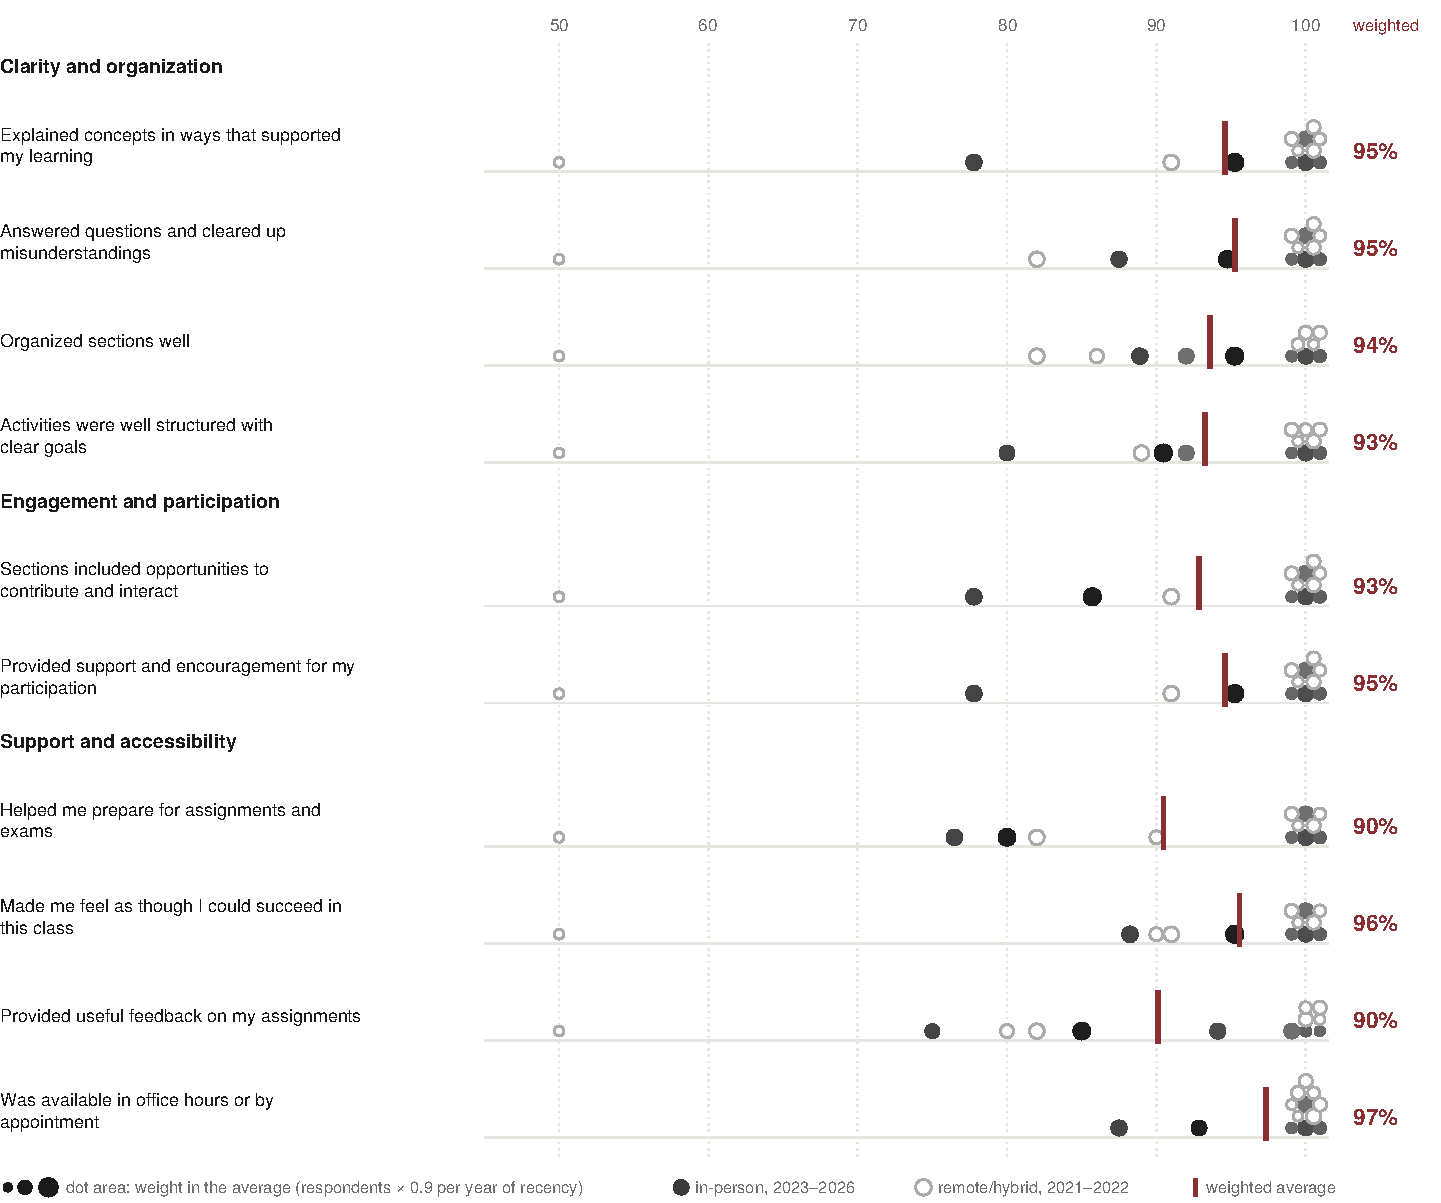
\includegraphics[width=0.85\linewidth]{evals_summary_figure_nokey.pdf}
\end{figure}

\subsection*{Instructor of record}

I taught Intermediate Microeconomics as a Graduate Student Instructor in Summer 2024 (online asynchronous; 11 of 37 students responded to the instructor survey).\footnote{The course was scheduled in person and moved to asynchronous online delivery two weeks before the term; I redesigned the materials and assessment sequence for that format.} Figure 2 reports every item on the instructor instrument, one dot per respondent: nine of nine respondents to the item said the problem sets prepared them for the examinations, and nine of eleven reported understanding the course's learning goals at the beginning of the course.

\begin{figure}[htbp!]
\captionsetup{labelformat=empty}
    \caption*{Figure 2: Instructor-of-record evaluation, Intermediate Microeconomics (Summer 2024). Each dot is one respondent.}
    \centering
    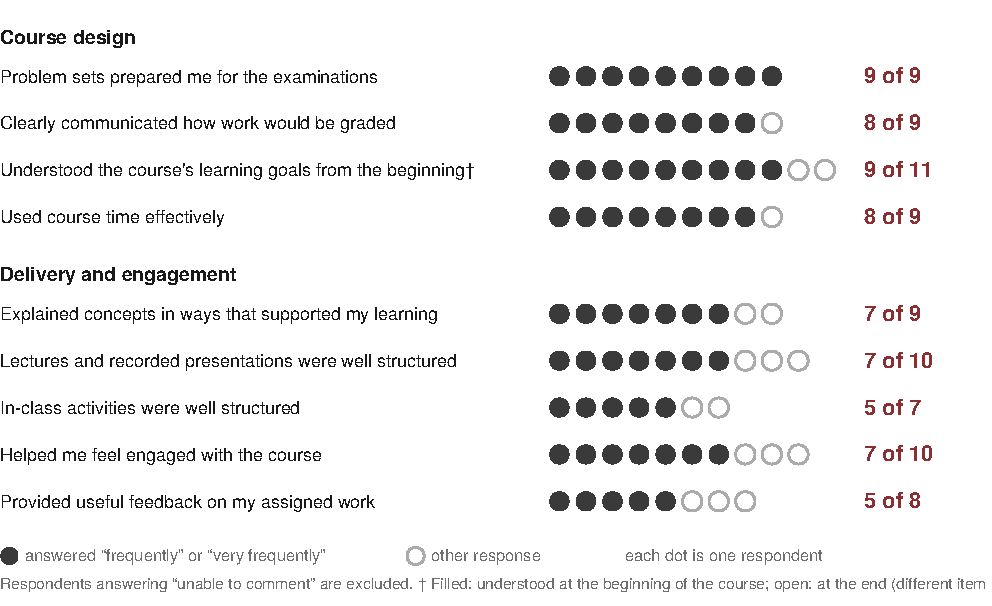
\includegraphics[width=0.8\linewidth]{gsi_figure.pdf}
\end{figure}

\subsection*{Selected comments}

All comments are quoted verbatim from the linked reports.

\begin{quote}\itshape ``I appreciated how interactive Gagandeep made sections. It was helpful that he encouraged every student interact instead of letting one or two students answer everything.'' \normalfont -- Applications in Microeconomics, Spring 2022\end{quote}
\begin{quote}\itshape ``Everyone in section was asked at least one question or another pertaining to the slides, which greatly helped with feeling engaged! If we got an answer wrong, Gagandeep was very encouraging and patient til we were able to find the correct solution -- it made the environment a lot less daunting. Additionally, the week of Thanksgiving when sections didn't meet, he sent us a recording of the material from the week on his own time. It was definitely the most engaging and enjoyable section I've been part of.'' \normalfont -- Introductory Macroeconomics, Fall 2023\end{quote}
\begin{quote}\itshape ``The TA made us try to answer to questions before giving us an explanation to make us try to think with our own minds first, and only afterwards we would be told the answer. I think this is really good.'' \normalfont -- Introductory Microeconomics, Winter 2026\end{quote}
\begin{quote}\itshape ``He was able to break down concepts in ways to where I actually understood course material instead of just going through the motions of solving problems using set equations.'' \normalfont -- Intermediate Microeconomics, Winter 2024\end{quote}
\begin{quote}\itshape ``I enjoyed how he encouraged us to participate in section, whether it was writing on the board or writing code on a collaborative Google Doc.'' \normalfont -- Applied Econometrics I (graduate), Fall 2024\end{quote}
\begin{quote}\itshape ``Gagandeep was one of the best teachers I have ever had. He is very passionate about what he does and cares about each and every student. He put in so much effort to create practice problems structured like our midterm questions. I do not think I would have done as well in this course without him.'' \normalfont -- Introductory Microeconomics, Winter 2026\end{quote}

\subsection*{Complete reports}

\begin{itemize}
    \item \href{https://gagandeep-sachdeva.com/teaching/TA_Evals_All_2020_2026.pdf}{Teaching assistant evaluations, all courses, 2020--2026}
    \item \href{https://gagandeep-sachdeva.com/teaching/teachingevals_GSI.pdf}{Instructor-of-record evaluation, Intermediate Microeconomics (Summer 2024)}
    \item \href{https://gagandeep-sachdeva.com/teaching/Feedback\%20for\%20TA\%20Workshops-\%20Fall\%202023.pdf}{Participant feedback, graduate TA pedagogy workshops (Fall 2023)}
    \item \href{https://gagandeep-sachdeva.com/teaching.html}{Teaching page}
\end{itemize}

\clearpage
\begin{table}[htbp!]
\captionsetup{labelformat=empty}
\caption*{Table 1: All courses. Item-group averages are the share of respondents answering ``frequently''/``very frequently,'' excluding ``unable to comment.''}
\centering
{\small
\begin{tabular}{llllrrrr}
\toprule
Quarter & Course & Modality & $n$ & RR & Clarity & Engag. & Support \\
\midrule
Winter 2026 & Introductory Microeconomics & In-person & 21 & 12\% & 94 & 90 & 88 \\
Winter 2025 & Introductory Microeconomics & In-person & 21 & 12\% & 84 & 78 & 82 \\
Fall 2024 & Applied Econometrics I (graduate) & In-person & 17 & 89\% & 100 & 100 & 98 \\
Spring 2024 & Intermediate Microeconomics & In-person & 9 & 8\% & 100 & 100 & 100 \\
Winter 2024 & Intermediate Microeconomics & In-person & 6 & 14\% & 100 & 100 & 100 \\
Fall 2023 & Introductory Macroeconomics & In-person & 17 & 11\% & 96 & 100 & 100 \\
Fall 2022 & Intermediate Microeconomics & Hybrid & 14 & 12\% & 86 & 91 & 89 \\
Spring 2022 & Applications in Microeconomics (graduate) & In-person & 2 & 15\% & 50 & 50 & 62 \\
Winter 2022 & Industrial Organization & Remote & 11 & 22\% & 96 & 100 & 100 \\
Fall 2021 & Intermediate Microeconomics & Remote & 3 & 7\% & 100 & 100 & 100 \\
Summer 2021 & Economic Rhetoric$^{\dagger}$ & Remote & 7 & 22\% & 100 & 100 & 100 \\
Spring 2021 & Introductory Microeconomics & Remote & 11 & 4\% & 100 & 100 & 100 \\
Winter 2021 & Introductory Microeconomics & Remote & 11 & 3\% & 100 & 100 & 90 \\
Spring 2025 & Introductory Macroeconomics$^{\ddagger}$ & In-person & -- & -- & -- & -- & -- \\
Winter 2020 & Introductory Microeconomics$^{\ddagger}$ & In-person & -- & -- & -- & -- & -- \\
\bottomrule
\end{tabular}}
\par\vspace{4pt}
{\footnotesize\raggedright $^{\dagger}$ Evaluated on an agree/disagree scale rather than the frequency scale. $^{\ddagger}$ Evaluation not available: Winter 2020 was administered on an earlier platform and could not be recovered; Spring 2025 is not available on the current platform.\par}
\end{table}

\end{document}